\PassOptionsToPackage{quiet}{fontspec}
\documentclass[UTF8,a4paper,12pt]{ctexart}

\usepackage{thesis}
\usepackage{amsmath}
\usepackage{amssymb}
\usepackage{booktabs}
\usepackage{caption}
\usepackage{subcaption}
\usepackage{graphicx}
\usepackage{float}
\usepackage{hyperref}
\usepackage{xcolor}
\usepackage{tabularx}
\usepackage{longtable}
\usepackage{enumitem}
\usepackage{placeins}
\usepackage{array}
\usepackage{tikz}
\usetikzlibrary{arrows.meta,positioning,shapes.geometric,fit,calc}

\graphicspath{{figures/}{figures/template_cover/}}
\newcolumntype{Y}{>{\raggedright\arraybackslash}X}
\hypersetup{
  colorlinks=true,
  linkcolor=blue!45!black,
  citecolor=blue!45!black,
  urlcolor=blue!45!black
}
\captionsetup{font=small,labelfont=bf}
\setlist{nosep}
\renewcommand{\arraystretch}{1.15}
\emergencystretch=2em
\setlength{\textfloatsep}{8pt plus 2pt minus 2pt}
\setlength{\floatsep}{8pt plus 2pt minus 2pt}
\setlength{\intextsep}{8pt plus 2pt minus 2pt}
\setlength{\abovecaptionskip}{4pt}
\setlength{\belowcaptionskip}{2pt}
\ctexset{
  section = {
    beforeskip = 1.0ex plus .2ex,
    afterskip = .6ex plus .1ex
  },
  subsection = {
    beforeskip = .8ex plus .2ex,
    afterskip = .4ex plus .1ex
  }
}
\setCJKmainfont{Noto Serif CJK SC}[BoldFont=Noto Serif CJK SC Bold]
\classname{量子线路路由编译实验}
\makepagestyle{}{}

\begin{document}
\setcounter{tocdepth}{2}

\maketitlepage{3230105807}
  {李浩瑄}
  {量子信息基础}
  {2026年6月}
  {钱浩亮}

\begingroup
\setstretch{1.02}
\addtocontents{toc}{\protect\enlargethispage{5\baselineskip}}
\maketoc
\endgroup

\section{摘要}

真实量子芯片通常只支持固定连接上的双比特门，而理想量子电路往往默认任意
逻辑量子比特都可以直接交互。量子路由编译的任务是在保持电路语义等价的前提
下，把逻辑量子比特映射到物理拓扑上，并插入必要的 SWAP 门，使电路能够在目标
硬件上合法执行。该问题可以表述为图约束下的映射与搜索问题，具有明显的组合
优化特征。

本项目实现了一条神经辅助量子路由流程 NPQR。该流程以神经网络动作为核心评分
信号，同时结合初始映射选择、有界束搜索、前沿触发、动作剪枝、局部后缀修复和
轨迹复放验证。SABRE 作为稳定的传统启发式基线，仅用于结果对比，不参与 NPQR
的路线生成。系统提供命令行、REST API、MCP 服务和网页演示入口，使算法能够被
直接调用和展示。

基于现有公开证据，项目已经完成可运行、可验证、可解释的组合式量子路由流程。
快速基线矩阵显示 SABRE 在不同启发式配置下具有稳定表现；项目证据同时表明
NPQR 能在固定困难样例上完成路由、返回可复放轨迹，并保持 REST API 与 MCP 调用
结果一致。本文报告算法建模、流程设计、系统实现、复杂度分析和结果边界。报告
不声称 NPQR 在所有电路上优于 SABRE，也不声称默认模型达到最先进量子路由水平。

\section{引言}

\subsection{实验背景}

量子计算的线路模型给出了一个清晰的抽象：量子寄存器保存量子态，量子门按时间顺序
作用在寄存器上，整个计算过程对应复向量空间中的酉演化。课程中讨论的叠加、纠缠、
测量、CNOT、QFT 和 QAOA 等概念，都可以在线路模型中得到统一描述。这个模型适合
讲清楚量子信息的数学结构，也适合作为算法设计的起点。

真实芯片给这个模型增加了硬件约束。以超导量子芯片为例，物理量子比特按固定拓扑
连接，双比特门只能在相邻物理量子比特之间直接执行。理想线路中的两个逻辑量子比特
可能在算法层面相互作用频繁，但映射到芯片后，它们未必位于相邻物理位置。编译器
需要在逻辑线路和物理拓扑之间建立对应关系，并在不相邻时插入 SWAP 重新安排量子态。
这一步不会改变理想语义，却会增加额外门操作。在线路深度增大后，退相干、门误差和
串扰带来的影响更明显，路由质量会直接影响量子程序在真实设备上的可执行性和可靠性。

量子线路路由因此成为一个典型的交叉问题。一方面，它建立在量子信息基础之上：每个
门都是对量子态的酉变换，SWAP 对应两个量子比特状态的交换，硬件拓扑限制了双比特
相互作用的物理位置。另一方面，它又是一个组合优化问题：编译器必须在大量可能映射
和候选 SWAP 中选择一条路径，使输出线路满足拓扑约束，同时尽量减少 SWAP 数、深度
和编译耗时。对于几十个量子比特的线路，简单枚举不可行，启发式搜索和学习辅助方法
具有实际意义。

\subsection{实验目标}

本项目从复现 SABRE 基线开始。SABRE 是量子路由中常用的启发式方法，它利用前沿门、
物理距离和后续门信息选择候选 SWAP，能够在较短时间内给出稳定结果。先实现并复现
这一基线，有两个作用：第一，它给出了传统方法的可比较参照；第二，它让后续自研
方法始终在同一线路、同一拓扑和同一指标下讨论，而不是只展示单独算法的绝对数值。

在此基础上，项目设计了 NPQR 学习评分路由方法。NPQR 并不把路由完全交给学习模型
决策，而是把模型放入显式搜索流程中：初始映射根据逻辑交互结构选择起点，动作掩码
缩小候选 SWAP 集合，模型评分给候选动作排序，束搜索保留多条可能路线，局部修复
处理尾部卡顿状态，轨迹复放验证每一步门是否满足硬件边约束。这样的设计保留了搜索
过程的可解释性，也使结果能够通过可视化回放和指标表格相互印证。

项目最终不只停留在算法脚本层面，而是实现为一个可演示、可运行、可复现的系统成果。
系统支持网页演示、服务器接口、工具接口和本地命令行；前端展示线路输入、拓扑映射、
SWAP 插入和指标对比；后端负责执行编译、返回结果并支持扩展实验。围绕这些交付形式，
项目补齐 README、测试、部署说明和报告材料，使代码实现、在线页面、服务接口和
本地示例形成统一交付。

\subsection{实验设计思路}

本文按“基础问题、基线复现、自研方法、系统交付、实验验证”的顺序展开。后文先介绍
量子比特、量子门、SWAP、硬件拓扑和路由目标，再说明 SABRE 基线的复现方法与实验
口径；随后给出 NPQR 的自然演进过程，并介绍系统界面、轨迹回放、部署方式和测试
验证；在过程说明部分，报告单独讨论 AI 协作在资料整理、开发、测试和写作中的使用
方法；实验部分集中呈现主实验、扩展实验、消融实验和耗时分析；最后总结课程知识、
算法实现、工程交付和后续优化方向。

\section{实验环境与问题建模}

本章把报告后续使用的量子信息概念和路由编译模型放在同一条线上说明。量子线路路由
不是普通图搜索的直接套用：算法每插入一个 SWAP，都对应量子态在物理载体上的交换；
算法每推进一个双比特门，都必须同时满足线路依赖关系和芯片耦合约束。把这一层关系
讲清楚，后面的 SABRE 复现、NPQR 设计和实验指标才有明确的物理含义。

\subsection{量子线路基础}

一个量子比特的纯态写作
\[
  |\psi\rangle=\alpha|0\rangle+\beta|1\rangle,\qquad
  |\alpha|^2+|\beta|^2=1 .
\]
这里 $|0\rangle$ 和 $|1\rangle$ 是计算基，$\alpha$、$\beta$ 是复振幅。测量得到
$0$ 或 $1$ 的概率分别为 $|\alpha|^2$ 和 $|\beta|^2$。多个量子比特组成寄存器后，
状态空间由张量积给出，$n$ 个量子比特对应 $2^n$ 维复向量空间。量子线路中的门操作
不是任意线性变换，而是保持内积和概率归一性的酉变换。

这一定义决定了路由编译的基本边界。编译器可以改变逻辑量子比特放置在哪个物理位置，
也可以插入语义明确的辅助门，但不能改变原线路描述的量子演化。换言之，路由输出的
线路必须和输入线路在逻辑语义上等价，只是执行时使用了不同的物理量子比特顺序和
额外的交换操作。

\subsubsection*{量子门与 SWAP}

单比特门作用在一个二维子空间上，常见例子包括 $X$、$H$ 和相位门。双比特门作用在
两个量子比特的张量积空间上，是产生和调控纠缠的关键。本项目关注的硬件约束主要
来自双比特门，因为真实芯片通常只允许相邻物理量子比特之间直接执行 CNOT 或 CZ。

SWAP 是路由编译中最重要的辅助门。它的作用可以写为
\[
  \mathrm{SWAP}|a\rangle|b\rangle=|b\rangle|a\rangle .
\]
在矩阵形式下，SWAP 是酉矩阵；在物理解释上，它交换两个物理位置上承载的逻辑量子
态。因此，若逻辑量子比特 $q_i$ 和 $q_j$ 当前不相邻，编译器可以沿硬件边插入若干
SWAP，把二者移动到相邻位置后再执行目标双比特门。这个过程保持理想线路语义，却
增加门数和深度。

\subsection{线路与硬件拓扑}

量子线路可以看成有序门列
\[
  C=(g_1,g_2,\ldots,g_m).
\]
单比特门只依赖其作用的一个逻辑量子比特；双比特门依赖两个逻辑量子比特的当前状态。
如果两个门作用在同一逻辑量子比特上，后一个门必须等待前一个门完成。这些先后关系
构成线路依赖结构。路由算法中的“前沿门”正是依赖已经满足、下一步可以尝试执行的门。

线路结构影响路由难度。GHZ 线路通常形成链式或星形纠缠，QFT 线路包含密集的长距离
双比特交互，QAOA 和 VQE 线路则由问题图或变分层决定交互模式。若交互图和硬件拓扑
形状接近，路由器可以少插入 SWAP；若逻辑交互跨越拓扑远端，编译器必须频繁移动
量子态。后续实验选择这些线路类型，就是为了覆盖不同交互结构下的路由行为。

\subsubsection*{硬件拓扑}

真实芯片的物理连接用图表示：
\[
  G=(V,E),
\]
其中 $V$ 是物理量子比特集合，$E$ 是可直接执行双比特门的耦合边。若
$(u,v)\in E$，映射到 $u$ 和 $v$ 上的两个逻辑量子比特可以直接执行双比特门；若
$(u,v)\notin E$，编译器必须先通过 SWAP 改变映射。

图 \ref{fig:hardware-topology} 给出本报告使用的两类拓扑示意。20 比特代表实验使用
Tokyo 风格耦合图，扩展实验使用二维网格。两类拓扑的共同点是连接稀疏：每个物理
量子比特只和少数邻居相连，远距离逻辑交互必须通过多次交换完成。系统会预先计算
物理距离 $d_G(u,v)$，即两个物理量子比特在耦合图中的最短路径长度，并把它作为
候选 SWAP 评分、前沿门代价和初始映射选择的重要依据：
\[
  d_G(u,v)=\mathrm{dist}_G(u,v).
\]

\begin{figure}[H]
  \centering
  \resizebox{\linewidth}{!}{%
  \begin{tikzpicture}[
  q/.style={circle, draw=blue!55!black, fill=blue!6, minimum size=0.58cm, font=\scriptsize},
  gridq/.style={circle, draw=gray!65!black, fill=gray!7, minimum size=0.48cm, font=\tiny},
  edge/.style={draw=gray!65, thick},
  label/.style={font=\small, align=center},
  note/.style={rectangle, draw=blue!40!black, fill=blue!3, rounded corners=2pt,
    text width=3.15cm, align=left, inner sep=5pt, font=\scriptsize}
]
  \node[label] at (1.2,2.35) {20Q 拓扑};
  \foreach \i/\x/\name in {0/0/v_0,1/1.1/v_1,2/2.2/v_2}
    \node[q] (a\i) at (\x,1.6) {$\name$};
  \foreach \i/\x/\name in {0/0/v_3,1/1.1/v_4,2/2.2/v_5}
    \node[q] (b\i) at (\x,0.65) {$\name$};
  \foreach \i/\x/\name in {0/0/v_6,1/1.1/v_7,2/2.2/v_8}
    \node[q] (c\i) at (\x,-0.3) {$\name$};
  \foreach \u/\v in {a0/a1,a1/a2,b0/b1,b1/b2,c0/c1,c1/c2,
    a0/b0,a1/b1,a2/b2,b0/c0,b1/c1,b2/c2,a0/b1,b1/c2}
    \draw[edge] (\u) -- (\v);

  \node[label] at (6.1,2.35) {网格拓扑};
  \foreach \i in {0,...,4} {
    \foreach \j in {0,...,2} {
      \node[gridq] (g\i\j) at (4.5+0.65*\i,0.35+0.65*\j) {};
    }
  }
  \foreach \i in {0,...,3} {
    \foreach \j in {0,...,2} {
      \pgfmathtruncatemacro{\next}{\i+1}
      \draw[edge] (g\i\j) -- (g\next\j);
    }
  }
  \foreach \i in {0,...,4} {
    \foreach \j in {0,...,1} {
      \pgfmathtruncatemacro{\next}{\j+1}
      \draw[edge] (g\i\j) -- (g\i\next);
    }
  }

  \node[note] at (9.35,1.2) {
    顶点表示物理量子比特，边表示可直接执行双比特门的耦合关系。路由器只允许在边上
    执行目标门或插入 SWAP。
  };
\end{tikzpicture}

  }
  \caption{硬件拓扑}
  \label{fig:hardware-topology}
\end{figure}

\subsection{映射与路由目标}

逻辑量子比特集合记为 $Q$。路由过程中的映射写作
\[
  \pi:Q\rightarrow V ,
\]
表示逻辑量子比特当前被放置到哪个物理位置。若双比特门
$g=(q_i,q_j)$ 满足
\[
  (\pi(q_i),\pi(q_j))\in E,
\]
该门可以在当前映射下直接执行。若条件不满足，路由器需要选择一条物理边 $(u,v)$
插入 SWAP，并交换这两个物理位置上承载的逻辑量子比特。设 $\pi'$ 是执行 SWAP 后的
新映射，则位于 $u$ 和 $v$ 的两个逻辑量子比特互换位置，其余逻辑量子比特保持不变。

图 \ref{fig:routing-model} 用一个小例子说明映射和 SWAP 的关系。逻辑线路中
$q_0$ 和 $q_2$ 需要执行 CNOT，但初始映射把它们放在不相邻的物理位置。编译器不能
直接执行该门，只能先在硬件边上插入 SWAP，让逻辑量子态沿拓扑移动。这个例子解释了
为什么路由不是简单地把每个逻辑门翻译成一个物理门：一次 SWAP 会改变后续所有门看到
的物理位置，当前选择和未来代价紧密耦合。

\begin{figure}[H]
  \centering
  \begin{tikzpicture}[
  font=\small,
  title/.style={font=\bfseries\small, align=center},
  note/.style={font=\scriptsize, align=center, text=black!72},
  qnode/.style={circle, draw=blue!60!black, fill=blue!7, minimum size=0.56cm, font=\scriptsize},
  vnode/.style={circle, draw=black!55, fill=gray!6, minimum size=0.58cm, font=\scriptsize},
  occ/.style={circle, draw=green!45!black, fill=green!10, minimum size=0.58cm, font=\scriptsize},
  gate/.style={rectangle, draw=blue!55!black, fill=blue!5, rounded corners=2pt,
    minimum width=1.34cm, minimum height=0.52cm, align=center, font=\scriptsize},
  swap/.style={rectangle, draw=orange!70!black, fill=orange!10, rounded corners=2pt,
    minimum width=1.34cm, minimum height=0.52cm, align=center, font=\scriptsize},
  arrow/.style={-{Latex[length=2mm]}, thick, draw=black!62},
  edge/.style={thick, draw=black!42}
]
  \node[title] at (-3.95,2.05) {逻辑线路};
  \node[qnode] (q0) at (-5.25,1.15) {$q_0$};
  \node[qnode] (q1) at (-4.15,1.15) {$q_1$};
  \node[qnode] (q2) at (-3.05,1.15) {$q_2$};
  \node[gate] (g1) at (-4.15,0.25) {目标门\\$CX(q_0,q_2)$};
  \draw[edge, blue!45!black] (q0) -- (q1);
  \draw[edge, blue!45!black] (q1) -- (q2);
  \draw[edge, blue!70!black] (q0) to[bend left=32] (q2);

  \node[title] at (0,2.05) {初始映射};
  \node[occ] (a0) at (-1.15,1.18) {$v_0/q_0$};
  \node[vnode] (a1) at (0,1.18) {$v_1$};
  \node[occ] (a2) at (1.15,1.18) {$v_2/q_2$};
  \draw[edge] (a0) -- (a1);
  \draw[edge] (a1) -- (a2);
  \node[note] at (0,0.27) {$q_0$ 与 $q_2$ 不相邻，\\双比特门不能直接执行};

  \node[title] at (3.95,2.05) {插入 SWAP};
  \node[vnode] (b0) at (2.80,1.18) {$v_0$};
  \node[occ] (b1) at (3.95,1.18) {$v_1/q_0$};
  \node[occ] (b2) at (5.10,1.18) {$v_2/q_2$};
  \draw[edge] (b0) -- (b1);
  \draw[edge] (b1) -- (b2);
  \draw[edge, orange!80!black, line width=1.2pt] (b0) -- node[below=3pt, font=\scriptsize] {SWAP} (b1);
  \node[note] at (3.95,0.27) {交换后 $q_0$ 与 $q_2$ 相邻，\\原始门可在硬件边上执行};

  \draw[arrow] (-2.35,1.16) -- (-1.55,1.16);
  \draw[arrow] (1.55,1.16) -- (2.35,1.16);
  \node[swap] at (0,-0.86) {路由目标：在保持原线路语义的前提下，减少额外 SWAP 和线路深度};
\end{tikzpicture}

  \caption{路由问题}
  \label{fig:routing-model}
\end{figure}

\subsubsection*{评价指标}

本项目使用三个主要指标衡量路由结果：SWAP 数、线路深度和编译耗时。SWAP 数表示
为满足拓扑约束额外插入了多少交换门，它直接反映路由带来的额外操作。线路深度表示
按依赖关系分层后需要多少时间步执行，深度越大，量子态在噪声环境中停留的时间越长。
编译耗时表示算法生成结果需要的时间，它决定在线演示、服务器接口和本地工具的响应
速度。

三者可以写成一个综合优化目标：
\[
  \min \; \alpha N_{\mathrm{swap}}+\beta D+\gamma T ,
\]
其中 $N_{\mathrm{swap}}$ 是插入 SWAP 数，$D$ 是路由后线路深度，$T$ 是编译耗时，
$\alpha,\beta,\gamma$ 用于表示不同指标的权重。实际系统不求解精确全局最优解，而是
在有限时间内寻找拓扑合法、语义等价、质量较好的可行线路。这个选择符合量子信息基础大作业的
实验目标：重点比较不同算法设计在相同线路和拓扑下的可执行结果，而不是把问题化为
一个难以在报告规模内完整求解的精确优化模型。

\subsection{课程知识对应}

表 \ref{tab:concept-mapping} 概括了课程知识和本项目实现之间的对应关系。该表的作用
不是把课程概念逐条罗列，而是说明路由编译为什么适合作为量子信息基础大作业主题：
它同时涉及量子态、酉门、纠缠线路、硬件约束、噪声影响和近似优化。

\begin{table}[H]
  \centering
  \caption{课程对应}
  \label{tab:concept-mapping}
  \begin{tabularx}{\linewidth}{lY}
    \toprule
    知识点 & 项目体现 \\
    \midrule
    量子态 & 线路中的门序列描述量子态演化，路由输出必须保持逻辑语义等价。\\
    张量积 & 多量子比特寄存器位于张量积空间，双比特门作用在两个子系统上。\\
    酉门 & CNOT、CZ、SWAP 都是酉门；额外 SWAP 改变承载位置，不改变理想演化。\\
    纠缠 & GHZ、QFT 等样例包含密集双比特交互，对硬件拓扑更敏感。\\
    拓扑 & 芯片耦合关系被建模为图，只有图边上的物理量子比特能直接执行双比特门。\\
    噪声 & 额外 SWAP 和更深线路会增加噪声暴露时间，减少交换门具有物理意义。\\
    优化 & 映射选择、候选 SWAP、搜索剪枝构成受约束的组合优化过程。\\
    验证 & 轨迹复放逐步检查门操作和映射变化，确认输出线路满足拓扑约束。\\
    \bottomrule
  \end{tabularx}
\end{table}


\section{SABRE 基线复现实验}

自研路由算法之前，报告先复现 SABRE。这样安排有两个原因：一是 SABRE 本身就是量子
线路映射领域常用的启发式方法，适合作为量子信息基础大作业的经典算法起点；二是后续 NPQR 的
效果需要放在同一批线路、同一类拓扑和同一组指标下讨论。没有稳定基线，单独报告
一个 SWAP 数很难说明算法质量。

\subsection{算法思路}

SABRE 的核心思想是围绕“前沿门”逐步改善映射。在线路依赖关系中，所有前驱已经
完成的门构成当前前沿。若前沿中的双比特门已经落在硬件边上，路由器直接执行该门；
若它的两个逻辑量子比特在当前映射下不相邻，路由器就在相关物理邻边中选择一个
SWAP，更新映射后继续检查前沿。

这个过程把路由问题转化为局部搜索。每一步不尝试枚举完整线路的所有映射序列，而是
用当前前沿门和少量后续门估计候选 SWAP 的价值。设前沿门集合为 $F$，当前映射为
$\pi$，硬件图距离为 $d_G$，一个常用的前沿距离代价可以写成
\[
  H_{\mathrm{front}}(\pi)=
  \sum_{(q_i,q_j)\in F} d_G\bigl(\pi(q_i),\pi(q_j)\bigr).
\]
若候选 SWAP 使这个代价下降，前沿门离可执行状态就更近。SABRE 的 lookahead 和
decay 变体会进一步考虑后续门或重复移动惩罚；basic 变体保留最直接的距离启发式，
适合作为固定、可复现的质量基线。

\subsection{任务定义}

候选 SWAP 不需要从全部物理边中盲目选择。SABRE 通常先找出与前沿门相关的逻辑量子
比特，再把这些逻辑量子比特当前所在物理位置的邻边作为候选集合。这样做减少了搜索
分支，也把每一步选择集中在最可能推进当前线路的位置。

候选动作的评价具有明显的“当前与未来”权衡。只看当前门时，最短路径上的某个 SWAP
往往很有吸引力；但这个 SWAP 可能把另一个即将参与后续门的逻辑量子比特移远。SABRE
的启发式价值在于，它用前沿门和扩展集合共同估计一个动作，而不是只为当前门走一步
最短路。这也是本项目后续设计自研方法时保留“前沿门”“候选动作”“物理距离”这些
概念的原因。

\subsection{复现设置}

本项目复现 SABRE 时采用固定口径。输入线路使用 OpenQASM 2 表示，硬件拓扑使用
Tokyo 风格耦合图；映射预处理先把逻辑量子比特放入目标拓扑，再执行 SABRE 路由。
路由阶段比较 basic、lookahead 和 decay 三种启发式，随机种子固定为 42，单次基线
使用 1 次 trial；输出统一统计完成状态、SWAP 数和线路深度。后续主实验中的
“SABRE basic”即采用这一固定口径。

表 \ref{tab:quick-matrix} 给出小规模复现结果。GHZ5 在三种启发式下均不需要额外
SWAP，说明其交互结构已经适配当前拓扑。QFT5 和 QFT10 的长距离双比特交互更多，
三种启发式之间出现差异；在 QFT10 上，lookahead 的 SWAP 数低于 basic，说明后续门
信息能改善局部选择。报告后续仍选 basic 作为主要对照，是因为它定义清晰、参数少，
更适合作为固定基线；lookahead 和 decay 则用于说明 SABRE 本身也存在启发式设计
空间。

\begin{table}[H]
  \centering
  \caption{SABRE 快速基线矩阵}
  \label{tab:quick-matrix}
  \begin{tabular}{llrrr}
    \toprule
    电路 & 启发式配置 & SWAP 数 & 深度 & 是否完成 \\
    \midrule
    GHZ5 & basic & 0 & 7 & 是 \\
    GHZ5 & lookahead & 0 & 7 & 是 \\
    GHZ5 & decay & 0 & 7 & 是 \\
    QFT5 & basic & 8 & 53 & 是 \\
    QFT5 & lookahead & 7 & 55 & 是 \\
    QFT5 & decay & 7 & 55 & 是 \\
    QFT10 & basic & 42 & 168 & 是 \\
    QFT10 & lookahead & 29 & 156 & 是 \\
    QFT10 & decay & 30 & 167 & 是 \\
    \bottomrule
  \end{tabular}
\end{table}


\subsection{结果分析}

SABRE 复现给后续工作提供了三层参照。第一，它验证了线路解析、拓扑建模、映射更新
和 SWAP 统计这条基本实验链路可以运行。第二，它提供了传统启发式的质量水平，使
NPQR 的 SWAP 数、深度和耗时可以在同一指标下比较。第三，它暴露了经典启发式的
局部性：当线路包含密集长距离交互时，单步启发式很容易受到当前前沿门支配。后续
方法章围绕初始映射、束搜索和模型评分展开，正是为了在保留 SABRE 可解释结构的
同时扩大搜索视野。

\section{算法设计}

NPQR 是一个神经辅助的组合式量子路由算法。它的核心不是单独的神经网络模型，而是
“神经网络评分 + 经典搜索控制”的整体流程。图 \ref{fig:npqr-flow} 展示了主要
步骤，算法 \ref{alg:npqr} 给出高层伪代码。

\begin{figure}[H]
  \centering
  \begin{tikzpicture}[
  font=\small,
  phasebox/.style={
    rectangle,
    rounded corners=2pt,
    draw=blue!55!black,
    fill=blue!6,
    align=center,
    minimum width=2.6cm,
    minimum height=0.78cm
  },
  verify/.style={
    rectangle,
    rounded corners=2pt,
    draw=green!45!black,
    fill=green!8,
    align=center,
    minimum width=2.6cm,
    minimum height=0.78cm
  },
  arrow/.style={-{Latex[length=2mm]}, thick, draw=gray!70!black}
]
  \node[phasebox] (input)   at (0,0)       {线路与拓扑};
  \node[phasebox] (pre)     at (3.4,0)     {图预处理};
  \node[phasebox] (mapping) at (6.8,0)     {初始映射};

  \node[phasebox] (beam)    at (6.8,-1.65) {束搜索};
  \node[phasebox] (score)   at (3.4,-1.65) {动作评分};
  \node[phasebox] (front)   at (0,-1.65)   {前沿推进};

  \node[phasebox] (repair)  at (0,-3.30)   {局部修复};
  \node[verify]   (replay)  at (3.4,-3.30) {复放验证};
  \node[verify]   (output)  at (6.8,-3.30) {线路与指标};

  \draw[arrow] (input) -- (pre);
  \draw[arrow] (pre) -- (mapping);
  \draw[arrow] (mapping) -- (beam);
  \draw[arrow] (beam) -- (score);
  \draw[arrow] (score) -- (front);
  \draw[arrow] (front) -- (repair);
  \draw[arrow] (repair) -- (replay);
  \draw[arrow] (replay) -- (output);
\end{tikzpicture}

  \caption{NPQR 神经辅助量子路由流程}
  \label{fig:npqr-flow}
\end{figure}

从职责划分看，NPQR 的每个模块都解决搜索中的一个具体问题。表
\ref{tab:component-roles} 概括了这些模块的输入、输出和作用。

\begin{table}[H]
  \centering
  \caption{组件职责}
  \label{tab:component-roles}
  \begin{tabularx}{\linewidth}{lYYY}
    \toprule
    模块 & 输入 & 输出 & 作用 \\
    \midrule
    依赖关系 & 门序列 & 前沿门、前驱关系 & 判断哪些门可以在当前状态推进。\\
    拓扑预处理 & 硬件耦合图 & 距离矩阵、边集合 & 为动作评分和合法性检查提供图特征。\\
    初始映射 & 逻辑交互图、物理拓扑 & 候选初始布局 & 降低后续 SWAP 搜索压力。\\
    动作筛选 & 当前映射、前沿门 & 候选 SWAP 集合 & 删除弱相关动作，控制分支数量。\\
    模型评分 & 状态特征、候选动作 & 动作偏好分数 & 为搜索提供学习得到的局部判断。\\
    束搜索 & 候选状态、累计得分 & 多条候选路线 & 保留多条高分路线，提升搜索质量。\\
    局部修复 & 接近完成的路线 & 修复后的尾部轨迹 & 处理少量剩余门停滞的情况。\\
    轨迹复放 & 执行轨迹、硬件拓扑 & 合法性检查结果 & 确认最终线路满足拓扑约束。\\
    \bottomrule
  \end{tabularx}
\end{table}


\subsection{图预处理与前沿门}

系统首先解析输入电路，提取门序列、量子比特集合和双比特门依赖关系。随后将目标
芯片表示为无向图，并计算物理量子比特之间的最短路径距离矩阵。该预处理把后续
多次距离查询变成常数时间访问，是典型的时空权衡。

在路由过程中，系统维护当前前沿门集合。若前沿双比特门在当前映射下已经相邻，
系统直接执行该门并推进门依赖；若不能执行，系统生成候选 SWAP 动作，并进入评分
与搜索流程。

\subsection{初始映射选择}

初始映射决定逻辑量子比特最开始放置在哪些物理量子比特上。若初始映射与电路的
交互结构匹配，后续需要的 SWAP 会减少。NPQR 会根据逻辑交互关系和物理拓扑生成
多个候选映射，并对候选进行排序。该步骤把原始电路路由问题转化为较好的搜索起点，
降低后续局部搜索的压力。

\subsection{神经网络动作评分}

在每个非终止状态下，神经网络根据当前映射、前沿门、物理距离和候选 SWAP 动作
输出动作偏好分数。该分数不直接决定完整答案，而是作为束搜索中的一个启发式信号。
这种设计使模型能够参与决策，同时避免模型一次性生成完整电路带来的不可控风险。

为了便于解释，可以把一个候选动作 $a$ 在状态 $s$ 下的综合评分写成
\[
  F(s,a)=\lambda_1 P_\theta(a\mid s)-\lambda_2 H_{\mathrm{frontier}}(s,a)
  -\lambda_3 C_{\mathrm{depth}}(s,a)-\lambda_4 C_{\mathrm{repeat}}(s,a),
\]
其中 $P_\theta(a\mid s)$ 表示神经网络给出的动作偏好，$H_{\mathrm{frontier}}$
表示前沿门距离启发式代价，$C_{\mathrm{depth}}$ 表示对深度增长的惩罚，
$C_{\mathrm{repeat}}$ 表示对重复无效移动的惩罚。实际系统可以使用等价的排序
逻辑；该公式强调的是：神经网络提供主要偏好，但最终决策仍受拓扑距离和搜索状态
共同约束。

\subsection{有界束搜索}

单步贪心容易因为局部最优而卡住。NPQR 使用有界束搜索保留多条候选路线。每次
展开时，系统对候选状态进行评分，只保留排名靠前的若干条路线继续搜索。束宽越大，
搜索质量通常越高，但时间和空间消耗也随之增加。

束搜索的关键在于把“当前最优动作”扩展为“当前较优路线集合”。设第 $t$ 层保留的
状态集合为 $\mathcal{B}_t$，系统会对每个 $s\in \mathcal{B}_t$ 展开若干动作并生成
候选集合 $\mathcal{C}_{t+1}$，然后按累计评分取前 $B$ 个状态：
\[
  \mathcal{B}_{t+1}=\mathrm{TopB}(\mathcal{C}_{t+1}).
\]
这样做牺牲了一部分运行时间，但能减少单步评分误差造成的不可逆失败。

\subsection{触发剪枝与局部修复}

对普通样例，过重搜索会增加不必要耗时；对交互密集或随机性强的样例，过轻搜索又
可能漏掉可行路线。NPQR 使用前沿触发规则识别更难的局部结构，只在必要时启用更强
的前沿搜索。同时，动作剪枝会删除明显较差的 SWAP 候选，控制搜索树分支数。

触发规则主要关注前沿门的拥塞程度、候选动作是否能接触关键前沿量子比特、以及
普通展开是否出现停滞。若状态表现为“前沿门距离长期不能下降”或“候选动作虽然得分
相近但影响范围不同”，系统会扩大对前沿相关动作的考虑范围。动作剪枝则保留与当前
前沿门、短路径和神经评分更相关的候选，避免在所有硬件边上无差别展开。

当一条路线已经完成大部分门但在末端卡住时，NPQR 会启用有界后缀修复。后缀修复
不是全局穷举，而是在有限深度内围绕剩余门进行局部搜索，用于补齐接近完成的路线。

\subsection{轨迹复放验证}

最终结果必须通过轨迹复放。系统会从初始映射开始重新模拟所有门和 SWAP，检查每
一步是否满足硬件边约束，并确认所有原始门都已执行。只有通过复放验证的路线才会
作为 NPQR 结果返回。该步骤把搜索输出转化为可审计的工程结果。

轨迹复放还用于区分“搜索过程看似完成”和“输出结果确实可执行”。如果某一步双比特
门不在硬件边上，或某个原始门没有被执行，复放都会失败。这个设计对课程项目很重要：
它把算法输出和硬件约束重新绑定，避免只报告一个未经验证的启发式分数。

\begin{figure}[H]
  \centering
  \begin{minipage}{0.94\linewidth}
  \begin{tabbing}
  \hspace{1.8em}\=\hspace{1.8em}\=\hspace{1.8em}\=\kill
  \textbf{算法 1：NPQR 神经辅助量子路由}\\
  \textbf{输入：}量子电路 $C$，硬件图 $G$，束宽 $B$，修复深度 $R$\\
  \textbf{输出：}路由后电路、SWAP 数、轨迹或失败标记\\
  1. 解析 $C$，构建门依赖和前沿门集合；\\
  2. 计算 $G$ 上的距离矩阵，生成初始映射候选；\\
  3. 将候选映射转化为初始搜索状态集合；\\
  4. \textbf{while} 存在未完成状态 \textbf{do}\\
  \> 4.1 执行所有当前可直接执行的前沿门；\\
  \> 4.2 若状态完成，进行轨迹复放并返回结果；\\
  \> 4.3 生成合法 SWAP 候选动作；\\
  \> 4.4 用神经网络和距离启发式为动作评分；\\
  \> 4.5 根据触发规则决定是否扩大前沿搜索；\\
  \> 4.6 剪枝弱动作，展开候选状态；\\
  \> 4.7 保留评分最高的 $B$ 个状态；\\
  \> 4.8 若状态接近完成但卡住，尝试深度不超过 $R$ 的后缀修复；\\
  5. \textbf{return} 失败标记。
  \end{tabbing}
  \end{minipage}
  \caption{NPQR 高层伪代码}
  \label{alg:npqr}
\end{figure}

\section{系统实现}

项目不仅实现了算法流程，还提供了面向使用者的多种调用方式。系统调用链路如图
\ref{fig:system-chain} 所示。网页、REST API、MCP 服务和命令行都可以触发同一
套编译流程，并返回路由后电路、SWAP 数、深度、耗时、轨迹和 SABRE 基线指标。

\begin{figure}[H]
  \centering
  \begin{tikzpicture}[
  node distance=0.75cm and 0.7cm,
  entry/.style={rectangle, rounded corners=2pt, draw=orange!65!black, fill=orange!8,
    align=center, minimum width=2.6cm, minimum height=0.78cm, font=\small},
  routeCore/.style={rectangle, rounded corners=2pt, draw=blue!60!black, fill=blue!6,
    align=center, minimum width=3.0cm, minimum height=0.85cm, font=\small},
  data/.style={rectangle, rounded corners=2pt, draw=green!45!black, fill=green!7,
    align=center, minimum width=3.0cm, minimum height=0.85cm, font=\small},
  arrow/.style={-{Latex[length=2mm]}, thick, draw=gray!70!black}
]
  \node[entry] (web) {网页演示};
  \node[entry, below=of web] (rest) {REST API};
  \node[entry, below=of rest] (mcp) {MCP 服务};
  \node[entry, below=of mcp] (cli) {命令行};

  \node[routeCore, right=2.0cm of rest] (request) {统一编译请求\\QASM 或示例};
  \node[routeCore, right=of request] (runtime) {NPQR 路由运行时};
  \node[data, above=of runtime] (model) {默认推理模型};
  \node[data, below=of runtime] (baseline) {SABRE 基线对比};
  \node[routeCore, right=of runtime] (result) {路由结果\\轨迹与指标};

  \draw[arrow] (web.east) -- (request.west);
  \draw[arrow] (rest.east) -- (request.west);
  \draw[arrow] (mcp.east) -- (request.west);
  \draw[arrow] (cli.east) -- (request.west);
  \draw[arrow] (request) -- (runtime);
  \draw[arrow] (model) -- (runtime);
  \draw[arrow] (runtime) -- (baseline);
  \draw[arrow] (runtime) -- (result);
  \draw[arrow] (baseline.east) -| (result.south);
\end{tikzpicture}

  \caption{系统调用链路}
  \label{fig:system-chain}
\end{figure}

\subsection{接口层}

REST API 适合网页和普通后端调用。用户可以提交内置示例名称或自定义 OpenQASM 2
文本，系统返回结构化 JSON 结果。MCP 服务适合工具客户端和自动化场景，能够查询
状态、列出示例、运行 NPQR、运行 SABRE 基线并返回算法证据。命令行适合本地检查、
演示和快速基线矩阵生成。

这些入口的共同点是都把 NPQR 作为默认编译流程，同时把 SABRE 作为对比结果返回。
接口中的对比字段用于解释基线表现，不表示 NPQR 失败时会由 SABRE 替代完成。

\subsection{编译层}

编译层负责把输入电路转化为路由任务，调用 NPQR 运行时，并将结果重新组织为用户
可读的输出。输出包括路由后 QASM、插入 SWAP 数、电路深度、运行时间和可复放轨迹。
轨迹字段使用户能够观察每一步 SWAP 和门执行，也便于报告中解释算法过程。

\subsection{模型与证据层}

项目包含一个默认推理模型。该模型在搜索循环中提供动作偏好，不单独承担完整路由
生成。系统还提供机器可读的算法证据，说明默认路由、算法组成、SABRE 基线、能力
边界和固定困难样例的闭环验证结果。该证据用于保证报告、网页和接口描述保持一致。

\section{项目部署与交付}

本章说明项目如何从本地算法实现变成可打开、可运行、可复现的量子信息基础大作业成果。交付
形态包括公开仓库、在线前端、服务器接口、协议工具、命令行、测试验证和报告 PDF。
这些材料共同支撑网页体验、接口调用和本地复现实验。

\subsection{项目组织}

公开仓库是项目总览。仓库首页说明项目目标、安装方式、在线演示、服务接口、命令行
用法、样例线路、拓扑选择和主要实验结果。报告 PDF、网页演示、示例线路、测试脚本
和说明文档都放在同一仓库中，避免出现“报告写了一套、代码在另一套环境中”的问题。

项目组织遵循量子信息基础大作业的交付逻辑：仓库说明项目目标和运行方式，在线前端呈现交互
效果，命令行和服务接口支持复现实验，公开测试维持说明、接口和示例的一致性。这个
结构把算法、系统和实验联系在一起。

图 \ref{fig:github-entry} 展示公开仓库入口。仓库首页把 README、许可证、目录结构、
在线前端和提交历史放在同一视图中，读者进入仓库后可以先阅读快速入口，再根据需要
打开网页、启动服务或运行本地测试。

\begin{figure}[H]
  \centering
  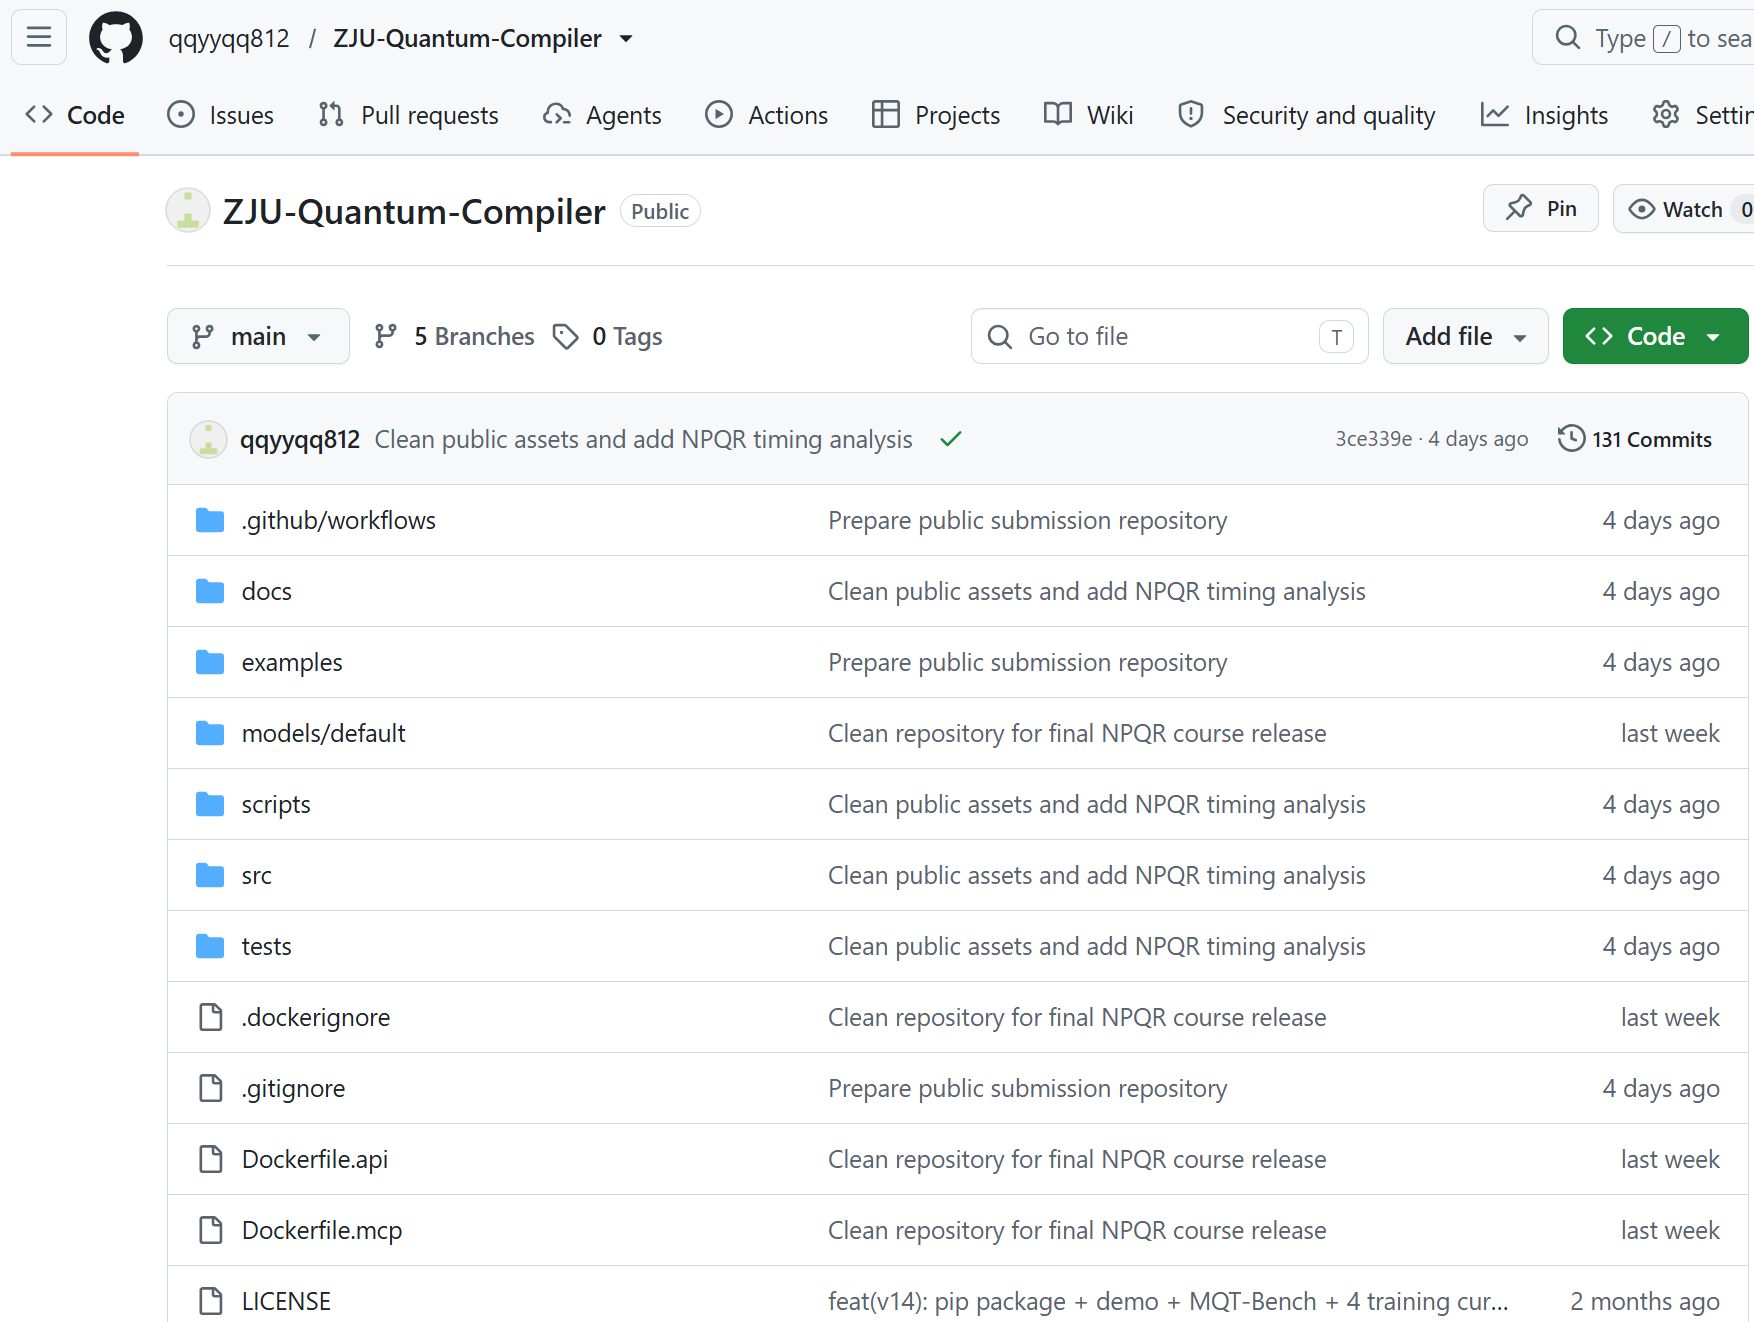
\includegraphics[width=0.92\linewidth]{figures/github-entry.png}
  \caption{仓库入口}
  \label{fig:github-entry}
\end{figure}

图 \ref{fig:project-timeline} 展示项目周期。整体工作先完成 SABRE 基线与最小路由
闭环，再围绕 NPQR 增加初始映射、模型评分、束搜索、修复和复放；随后把算法封装为
网页、REST、MCP 和命令行；最后整理公开仓库、在线前端、服务器服务、测试验证和
报告材料。

\begin{figure}[H]
  \centering
  \begin{tikzpicture}[
  node distance=0.45cm,
  stage/.style={
    rectangle,
    draw=blue!45!black,
    fill=blue!4,
    rounded corners=2pt,
    text width=0.18\linewidth,
    align=left,
    inner sep=5pt,
    font=\footnotesize
  },
  arrow/.style={-{Latex[length=2.2mm]}, thick, draw=blue!45!black}
]
\node[stage] (s1) {
  \textbf{阶段一}\\
  基线闭环\\
  QASM、拓扑、SABRE、最小路由任务
};
\node[stage, right=0.45cm of s1] (s2) {
  \textbf{阶段二}\\
  NPQR 迭代\\
  初始映射、模型评分、束搜索、修复
};
\node[stage, right=0.45cm of s2] (s3) {
  \textbf{阶段三}\\
  系统封装\\
  REST、MCP、CLI、前端控制台
};
\node[stage, right=0.45cm of s3] (s4) {
  \textbf{阶段四}\\
  交付整理\\
  GitHub Pages、华为云、报告与测试
};
\draw[arrow] (s1) -- (s2);
\draw[arrow] (s2) -- (s3);
\draw[arrow] (s3) -- (s4);
\end{tikzpicture}

  \caption{项目周期}
  \label{fig:project-timeline}
\end{figure}

\subsection{在线前端}

前端采用静态网页发布，适合课程展示和跨设备访问。静态页面不要求访问者先配置本地
环境，打开后即可查看示例、拓扑、指标面板和轨迹回放。当服务器接口可达时，页面
会把编译请求发送到后端；当读者只想了解功能时，页面中的样例和说明也能独立展示
项目结构。

GitHub Pages 适合承载这类公开展示页面：它与公开仓库天然绑定，更新流程清晰，访问链接
固定。前端不保存实验结论本身，而是作为编译结果
的展示层；真正的路由、基线比较和轨迹生成仍由共享编译核心完成。

\subsection{服务器部署}

服务器部署负责处理真实编译请求。后端服务接收线路、后端选择和拓扑名称，调用同一
编译核心，并返回路由后线路、指标和轨迹。服务端提供健康状态、样例列表、拓扑查询、
线路校验、同步编译、异步任务和实验摘要等能力。异步任务用于耗时稍长的线路，避免
浏览器在等待过程中失去响应。

云端部署使用容器化方式固定运行环境。这样做有两个优点：一是依赖库、模型文件和
服务启动方式可以被明确记录；二是本地运行和服务器运行使用同一套调用方式，减少“本地
能跑、线上不一致”的问题。报告中的在线前端与服务器接口保持分工：前端负责交互，
服务器负责计算。

\subsection{工具接口}

除普通网页和 REST 调用外，项目还提供 MCP 与命令行两类接口。MCP 面向支持工具调用
的客户端，适合把量子编译能力接入自动化工作流；命令行面向本地复现，用于确认
安装状态、编译内置样例和生成对照矩阵。

这两类接口的价值在于扩展使用场景。网页适合展示，REST 适合应用集成，MCP 适合工具
编排，命令行适合复现实验。四种调用方式共享同一结果字段，因此不会形成互相矛盾的结果
口径。

\subsection{测试与复现}

公开交付包含一组基础测试。测试覆盖服务契约、网页静态契约、
README 内容、部署配置和材料完整性。这里的测试目标不是证明算法在所有可能线路上
最优，而是保证说明、接口和示例能够互相对应。

表 \ref{tab:delivery-checklist} 汇总主要交付项。正文只解释交付结构，具体命令放在
附录中，作为复现实验的命令说明。

\begin{table}[H]
  \centering
  \caption{交付清单}
  \label{tab:delivery-checklist}
  \begin{tabularx}{\linewidth}{lY}
    \toprule
    交付项 & 作用 \\
    \midrule
    公开仓库 & 汇总代码、报告、样例、测试和说明文档。\\
    在线前端 & 展示线路输入、拓扑选择、轨迹回放和指标对比。\\
    服务器接口 & 处理真实编译请求，返回路由线路、指标和轨迹。\\
    MCP 服务 & 为工具客户端提供状态查询、样例读取和编译调用能力。\\
    命令行接口 & 支持本地安装确认、示例编译和对照矩阵生成。\\
    测试验证 & 覆盖公开接口、网页契约、README 和材料完整性。\\
    报告 PDF & 汇总理论基础、SABRE 复现、NPQR 方法、系统部署和实验结果。\\
    \bottomrule
  \end{tabularx}
\end{table}


\section{AI 辅助开发}

本项目把 AI 工具作为工程协作环境的一部分，而不是把它作为算法结论的来源。量子线路
路由同时涉及量子信息、图搜索、学习模型、前后端接口和部署流程，单靠一次性编写代码
很难把这些部分稳定连接起来。AI 的作用主要体现在信息整理、方案比较、代码阅读、界面
修订和文档组织上；项目目标、算法取舍、实验口径和最终文字由作者根据课程要求和实际
运行结果确定。

\subsection{资料整理}

项目早期需要把课程知识、经典路由算法和工程实现放在同一问题框架中。AI 辅助完成的
第一类工作是资料整理：把量子态、酉门、双比特门、SWAP、硬件耦合图和线路深度这些
课程概念对应到路由编译任务；把 SABRE 的前沿门、候选交换和距离启发式整理成可复现
的基线描述；再把 NPQR 的初始映射、束搜索、动作评分和轨迹复放放到“学习评分搜索”
这一叙事下。

这种整理不是替代阅读论文，而是帮助形成报告结构。SABRE、图神经网络辅助路由和强化
学习路由等相关方法提供了参考坐标：传统启发式强调速度和稳定性，学习方法强调从局部
结构中学习动作偏好，搜索框架负责保证拓扑约束和状态推进。本项目最终选择的写法是先
复现 SABRE，再说明自研方法如何在同一实验口径下逐步改进。

\subsection{网页开发}

网页演示需要让读者直观看到量子路由的过程，而不是只看到一个数字表格。AI 在前端部分
主要用于交互方案和界面细节的讨论：输入区如何容纳 OpenQASM，拓扑图和指标面板如何
并列显示，轨迹回放如何同步显示 SWAP、物理边和逻辑位交换，错误信息如何写得清楚但
不干扰主流程。

前端技术栈保持简单：静态页面负责展示和交互，浏览器脚本负责请求服务接口、渲染拓扑、
回放轨迹和更新指标。这样的选择适合量子信息基础大作业，因为它不要求额外的前端构建流程，并且
可以直接通过 GitHub Pages 发布。AI 辅助的价值主要体现在快速比较布局方案、核对按钮状态、
梳理响应字段和改写界面文案；最终页面是否可用，仍由实际浏览器打开、接口调用和样例
回放决定。

\subsection{服务开发}

后端服务承担真实编译任务。AI 在这一部分更多地用于代码阅读和接口一致性梳理：
梳理 REST、MCP 和命令行三种调用方式需要共享哪些字段，整理状态查询、示例列表、线路校验、
同步编译、异步任务和拓扑查询之间的返回格式是否一致，帮助发现前端字段和后端响应之间
的不匹配。

服务端技术栈包括 Python、FastAPI、Uvicorn、Qiskit、PyTorch、NetworkX 和 Rustworkx。
其中 Qiskit 用于量子线路处理和 SABRE 基线，图工具用于硬件拓扑和距离计算，PyTorch
用于模型评分模块，FastAPI 和 Uvicorn 用于把编译能力暴露为服务。AI 辅助在这里更像
一名工程搭档：它可以根据接口约定整理验证项，但每一次接口修改都需要通过实际请求、
测试用例和网页调用来确认。

\subsection{部署测试}

部署阶段容易出现两类问题：一类是本地可运行但服务器环境缺少依赖，另一类是 README、
网页、接口和测试之间的说明不一致。AI 在这一阶段用于整理验证流程，例如服务健康状态、
样例编译、静态页面契约、公开测试和材料完整性。容器化服务、GitHub Pages 和公开仓库
共同构成了本项目的交付链路。

这一过程也帮助项目把“能运行”扩展为“能交付”。本地命令行适合快速复现实验，REST
服务适合网页和脚本调用，MCP 适合工具客户端集成，GitHub Pages 适合课程展示。AI 可以
辅助列出这些调用方式之间需要保持一致的结果字段，但真正的通过标准是服务能够启动、网页
能够调用、测试能够运行、报告中的实验数据能够对应到实际输出。

\subsection{报告整理}

报告写作阶段，AI 主要用于结构重组和文字修订。早期材料更像项目说明，包含较多接口、
路径和过程记录；正式报告需要改成量子信息基础大作业文风：先讲量子信息基础和硬件约束，再讲
SABRE 复现、自研方法、系统部署和实验对照。AI 在这里帮助发现章节之间的断裂，例如
摘要是否回应课程要求，图表标题是否过长，实验结论是否对应表格，系统与部署是否混在
同一节中。

最终写法遵循两个原则。第一，正文解释问题和方法，具体复现命令放到附录；第二，图表
标题保持简短，详细解释放在段落中。这样可以减少工程文件列表对正文节奏的干扰，让报告
更接近课程论文，而不是开发日志。

\subsection{过程控制}

AI 协作最关键的部分是控制权。作者负责确定量子信息基础大作业的目标、选定对照基线、决定哪些
实验进入正文、运行测试和编译 PDF，并对最终结论负责。AI 给出的代码方案、文字方案和
实验组织方案只有在符合实际代码、样例输出和课程要求时才会被采用。

因此，本项目中的 AI 使用方式可以概括为：用 AI 提高阅读、开发和整理效率，用代码运行
结果决定结论。对于量子线路路由这样涉及算法与工程闭环的问题，这种协作方式能够减少
重复劳动，也能帮助报告保持清晰结构；但项目可信度仍来自可运行系统、可复现实验和明确
的课程知识对应关系。

\section{实验结果与数据分析}

实验部分围绕三个问题展开。第一，NPQR 在代表性线路上是否能生成通过复放的路由
结果。第二，在同一线路和同一拓扑下，NPQR 相比 SABRE basic 能减少多少 SWAP。
第三，初始映射、束搜索、模型评分和局部修复这些设计在运行成本和结果质量上分别
起到什么作用。

\subsection{实验设置}

主实验采用固定对照口径。20 比特以内线路使用 Tokyo 20Q 拓扑，30/50 比特扩展线路
使用规则网格拓扑；NPQR 与 SABRE basic 使用相同输入线路、相同拓扑和相同指标字段。
SABRE basic 作为固定基线，只用于质量比较；NPQR 路线由自研流程生成，并经过轨迹
复放后进入表格。

\begin{table}[H]
  \centering
  \caption{实验指标说明}
  \label{tab:metrics}
  \begin{tabularx}{\linewidth}{lYY}
    \toprule
    指标 & 含义 & 解释方式 \\
    \midrule
    完成状态 & 是否成功生成满足约束的路由结果 & 是底线指标，未完成时 SWAP 和深度比较意义有限。 \\
    SWAP 数 & 插入的交换门数量 & 越低通常表示路由额外开销越小。 \\
    电路深度 & 路由后门序列的层数 & 越低通常表示潜在执行时间和噪声暴露越少。 \\
    运行时间 & 编译请求耗时 & 越低越适合在线接口和课堂演示。 \\
    轨迹复放 & 按输出轨迹重新验证拓扑合法性 & 用于确认结果不是仅由启发式分数推断。 \\
    基线差异 & 与 SABRE 指标的对照 & 用于观察算法表现边界，不作为唯一成功标准。 \\
    \bottomrule
  \end{tabularx}
\end{table}


实验指标见表 \ref{tab:metrics}。完成状态是先决指标：只有所有原始门被执行、每个
双比特门都满足硬件边约束、轨迹可以从初始映射复放到最终映射时，结果才记为完成。
在完成前提下，SWAP 数衡量额外交换开销，线路深度衡量可并行执行层数，运行时间衡量
在线演示和批量复现实验的计算成本。

\subsection{基础实验}

10/20 比特实验是本报告的主要质量证据。样例覆盖 GHZ、QFT、QAOA、VQE、随机线路
和结构化 20 比特线路，分别对应链式纠缠、长程交互、局部哈密顿量结构、变分线路和
较不规则的双比特门分布。

\begin{table}[H]
  \centering
  \caption{10/20 比特代表电路与 SABRE basic 的最终对比}
  \label{tab:final-basic-matrix}
  \begin{tabular}{lrrrr}
    \toprule
    电路 & 比特数 & NPQR SWAP & SABRE basic SWAP & 差值 \\
    \midrule
    GHZ10 & 10 & 2 & 6 & -4 \\
    QFT10 & 10 & 6 & 13 & -7 \\
    QAOA10 & 10 & 0 & 15 & -15 \\
    VQE10 & 10 & 1 & 4 & -3 \\
    Random10 & 10 & 17 & 19 & -2 \\
    Brickwork20 & 20 & 15 & 31 & -16 \\
    CliqueBlocks20 & 20 & 19 & 38 & -19 \\
    DeepRandom20 & 20 & 105 & 135 & -30 \\
    RingEntangler20 & 20 & 16 & 41 & -25 \\
    SparseRandom20 & 20 & 37 & 57 & -20 \\
    \bottomrule
  \end{tabular}
\end{table}


表 \ref{tab:final-basic-matrix} 显示，NPQR 在 10 个代表样例上全部完成路由，SWAP
数均低于 SABRE basic。10 个样例合计，NPQR 插入 218 个 SWAP，SABRE basic 插入
359 个，减少 141 个，降幅为 39.3\%。其中 10 比特样例从 57 个降至 26 个，20 比特
样例从 302 个降至 192 个。

图 \ref{fig:swap-comparison} 选取不超过 70 个 SWAP 的代表行画成柱状图，避免
DeepRandom20 这类大值压缩其他样例的视觉差异。结构化线路的收益最明显：QAOA10
从 15 个 SWAP 降至 0 个，CliqueBlocks20 从 38 个降至 19 个，RingEntangler20 从
41 个降至 16 个。随机线路的改善幅度相对小一些，但仍保持同向：Random10 减少
2 个 SWAP，SparseRandom20 减少 20 个 SWAP。这说明 NPQR 的收益并不只来自某一个
特定样例，而是同时出现在结构化线路和随机线路中。

\begin{figure}[H]
  \centering
  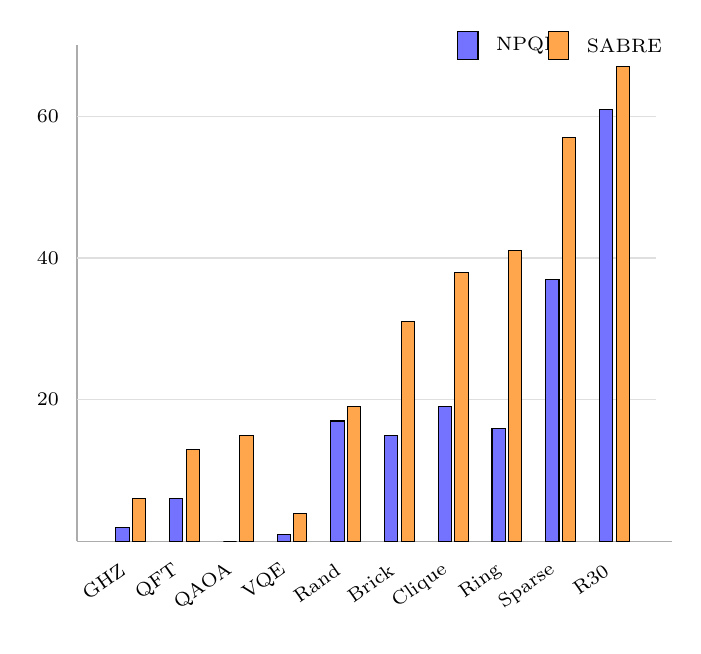
\begin{tikzpicture}[
  x=1.05cm,
  y=0.09cm,
  font=\scriptsize,
  axis/.style={draw=gray!65},
  npqr/.style={fill=blue!55},
  sabre/.style={fill=orange!70}
]
  \draw[axis] (0,0) -- (7.2,0);
  \draw[axis] (0,0) -- (0,70);
  \foreach \y in {20,40,60} {
    \draw[gray!25] (0,\y) -- (7.0,\y);
    \node[anchor=east] at (-0.1,\y) {\y};
  }

  \def\npqrvals{2,6,0,1,17,15,19,16,37,61}
  \def\sabrevals{6,13,15,4,19,31,38,41,57,67}
  \foreach \n [count=\i from 1] in \npqrvals {
    \pgfmathsetmacro{\x}{0.65*\i}
    \draw[npqr] (\x-0.18,0) rectangle (\x-0.02,\n);
  }
  \foreach \s [count=\i from 1] in \sabrevals {
    \pgfmathsetmacro{\x}{0.65*\i}
    \draw[sabre] (\x+0.02,0) rectangle (\x+0.18,\s);
  }

  \foreach \label [count=\i from 1] in {GHZ,QFT,QAOA,VQE,Rand,Brick,Clique,Ring,Sparse,R30} {
    \pgfmathsetmacro{\x}{0.65*\i}
    \node[rotate=35, anchor=east] at (\x,-3) {\label};
  }
  \draw[npqr] (4.6,68) rectangle (4.85,72);
  \node[anchor=west] at (4.95,70) {NPQR};
  \draw[sabre] (5.7,68) rectangle (5.95,72);
  \node[anchor=west] at (6.05,70) {SABRE};
\end{tikzpicture}

  \caption{SWAP 对比}
  \label{fig:swap-comparison}
\end{figure}

\subsection{拓展实验}

扩展实验选择 30/50 比特网格样例，用来观察同一套路由流程在更大拓扑上的表现。这里
不把扩展样例作为全规模能力结论，而是作为补充实验：线路规模增大后，初始映射和搜索
仍需在受限耦合图上给出可复放路线。

\begin{table}[H]
  \centering
  \caption{扩展实验}
  \label{tab:scale-smoke}
  \begin{tabular}{lrrrr}
    \toprule
    线路 & 比特数 & NPQR SWAP & SABRE basic SWAP & 差值 \\
    \midrule
    LineGHZ30 & 30 & 23 & 43 & -20 \\
    Random30-d4 & 30 & 61 & 67 & -6 \\
    LineGHZ50 & 50 & 50 & 79 & -29 \\
    RingSparse50 & 50 & 98 & 113 & -15 \\
    \bottomrule
  \end{tabular}
\end{table}


表 \ref{tab:scale-smoke} 中 4 个扩展样例全部完成，且 SWAP 数均低于 SABRE basic。
LineGHZ30 从 43 个 SWAP 降至 23 个，LineGHZ50 从 79 个降至 50 个；这类链式纠缠
线路受益于较好的初始布局。Random30-d4 和 RingSparse50 的改善幅度较小，分别减少
6 个和 15 个 SWAP，说明在较不规则交互下，NPQR 仍能形成优势，但搜索压力更高。

\subsection{消融实验}

消融实验采用 10 比特子集，固定 Tokyo 20Q 拓扑和相同最大步数，只改变路由组件。
该组实验用于观察模块作用，不替代主实验结论。完整配置包含结构化初始映射、多候选
束搜索和模型动作评分；单步选择把束宽和分支数都降为 1；简单映射减少初始映射候选
和局部布局优化。

\begin{table}[H]
  \centering
  \caption{消融实验}
  \label{tab:ablation-study}
  \begin{tabularx}{\linewidth}{lrrY}
    \toprule
    配置 & 完成数 & 完成样例 SWAP 合计 & 观察 \\
    \midrule
    完整配置 & 4/4 & 23 & GHZ10、QFT10、QAOA10、VQE10 全部完成。\\
    单步选择 & 1/4 & 0 & 只完成 QAOA10，长程交互样例容易停滞。\\
    简单映射 & 2/4 & 22 & QFT10 和 QAOA10 完成，但 QAOA10 需要额外 SWAP。\\
    \bottomrule
  \end{tabularx}
\end{table}


表 \ref{tab:ablation-study} 显示，完整配置在 4 个样例上全部完成。去掉多候选保留后，
只有 QAOA10 完成；GHZ10、QFT10 和 VQE10 都在有限步数内停住。弱化初始映射后，
完成数提高到 2 个，但 GHZ10 和 VQE10 仍未完成，QAOA10 的 SWAP 数也从 0 增加到
3。这个结果支持方法章节中的判断：束搜索负责避免过早陷入局部路线，结构化映射负责
降低搜索起点的距离代价。

模型评分另做了动作价值信号分析。对 15 组正负路线状态，模型在 12 组中给可取路线
更高分，正向比例为 80\%，平均分差为 0.00213。这个数值不直接等同于 SWAP 降幅，
但说明模型评分具有可用于排序的局部信号；最终路线质量仍由动作掩码、束搜索、修复
和复放共同决定。

\subsection{运行过程}

为了解释运行成本，项目对 NPQR 主流程做了分阶段计时。计时覆盖预处理、依赖关系、
拓扑距离矩阵、逻辑交互图、初始映射候选、主搜索、动作生成、模型推理、束搜索
剪枝、后处理、局部修复和轨迹复放。表 \ref{tab:phase-timing} 选取三个代表样例：
QAOA10、QFT10 和 Brickwork20。

\begin{table}[H]
  \centering
  \caption{阶段耗时}
  \label{tab:phase-timing}
  \begin{tabularx}{\linewidth}{lrlrY}
    \toprule
    样例 & 规模 & 总耗时 & 最耗时阶段 & 搜索子阶段观察 \\
    \midrule
    QAOA10 & 10Q & $623.9\mathrm{ms}\pm61.2\mathrm{ms}$ &
    初始映射候选生成 92.6\% & 结构化线路主要由初始映射吸收路由成本。\\
    QFT10 & 10Q & $16.23\mathrm{s}\pm1.14\mathrm{s}$ &
    主搜索阶段 90.2\% & 模型推理约 7.75s，束搜索扩展与剪枝约 5.65s。\\
    Brickwork20 & 20Q & $13.35\mathrm{s}\pm0.86\mathrm{s}$ &
    初始映射候选生成 99.8\% & 20Q 候选映射成为主要成本。\\
    \bottomrule
  \end{tabularx}
\end{table}

图 \ref{fig:timing-distribution} 展示三类样例的瓶颈差异。QAOA10 和 Brickwork20 的
耗时集中在初始映射候选生成，说明结构化交互线路的主要成本在起点选择；QFT10 的主
搜索占 90.2\%，其中模型推理和束搜索扩展是主要子项。这个结果与复杂度分析一致：
当线路包含更多长程依赖时，候选状态数量和动作评分次数会成为主要增长项。

\begin{figure}[H]
  \centering
  \begin{tikzpicture}[
  x=1.6cm,
  y=0.055cm,
  font=\scriptsize,
  axis/.style={draw=gray!65},
  init/.style={fill=blue!55},
  search/.style={fill=orange!70},
  other/.style={fill=gray!35}
]
  \draw[axis] (0,0) -- (5.2,0);
  \draw[axis] (0,0) -- (0,105);
  \foreach \y in {25,50,75,100} {
    \draw[gray!25] (0,\y) -- (4.9,\y);
    \node[anchor=east] at (-0.08,\y) {\y\%};
  }

  \draw[init] (0.65,0) rectangle (1.05,92.6);
  \draw[search] (1.05,0) rectangle (1.45,4.0);
  \draw[other] (1.45,0) rectangle (1.85,3.4);
  \node[anchor=north] at (1.25,-3) {QAOA10};

  \draw[init] (2.15,0) rectangle (2.55,4.0);
  \draw[search] (2.55,0) rectangle (2.95,90.2);
  \draw[other] (2.95,0) rectangle (3.35,5.8);
  \node[anchor=north] at (2.75,-3) {QFT10};

  \draw[init] (3.65,0) rectangle (4.05,99.8);
  \draw[search] (4.05,0) rectangle (4.45,0.1);
  \draw[other] (4.45,0) rectangle (4.85,0.1);
  \node[anchor=north] at (4.25,-3) {Brick20};

  \draw[init] (1.05,106) rectangle (1.3,111);
  \node[anchor=west] at (1.38,108.5) {初始映射};
  \draw[search] (2.2,106) rectangle (2.45,111);
  \node[anchor=west] at (2.53,108.5) {主搜索};
  \draw[other] (3.15,106) rectangle (3.4,111);
  \node[anchor=west] at (3.48,108.5) {其他};
\end{tikzpicture}

  \caption{耗时分布}
  \label{fig:timing-distribution}
\end{figure}

实验总体说明，NPQR 的质量收益来自多个组件的组合，而不是单一技巧。初始映射减少
搜索起点的拓扑距离，束搜索保留多条候选路线，模型评分提供局部动作偏好，局部修复
处理尾部停滞，轨迹复放保证结果可验证。运行时间仍有优化空间，尤其是候选映射生成、
模型推理和束搜索扩展；这些开销也为后续批处理推理、候选剪枝和分层路由提供了明确
方向。

\section{实验讨论}

本节把 NPQR 的工程实现回扣到算法分析和量子信息基础知识。报告的重点不是堆叠公式，
而是说明为什么某些阶段耗时高、为什么 SWAP 数和线路深度有物理意义，以及本项目与
课程内容之间的对应关系。

\subsection{复杂度}

令 $n=|V|$ 表示物理量子比特数，$m$ 表示线路门数，$e=|E|$ 表示硬件边数，$K$
表示初始映射候选数，$B$ 表示束宽，$D$ 表示主搜索最大展开深度，$A$ 表示每个状态
保留的候选动作数，$R$ 表示后缀修复深度。NPQR 的主要成本来自候选映射、动作生成
与掩码、模型推理、束搜索扩展和局部修复。

\begin{table}[H]
  \centering
  \caption{复杂度}
  \label{tab:complexity}
  \begin{tabularx}{\linewidth}{lYY}
    \toprule
    阶段 & 时间复杂度估计 & 说明 \\
    \midrule
    拓扑距离矩阵 & $O(n^3)$ 或 $O(n(e+n\log n))$ & 取决于 Floyd 或多源最短路；固定拓扑下可复用。\\
    线路依赖图构建 & $O(m)$ & 扫描门序列，维护前沿门和执行依赖。\\
    逻辑交互图构建 & $O(m)$ & 统计双比特门交互强度，服务初始映射。\\
    初始映射候选 & $O(K\cdot n^2)$ 量级 & 与候选数量和映射评分方式有关。\\
    动作生成与掩码 & $O(B\cdot e)$ & 每个保留状态在硬件边上筛选候选 SWAP。\\
    模型推理 & $O(B\cdot A\cdot C_\theta)$ & $C_\theta$ 为单次模型评分成本。\\
    束搜索扩展 & $O(D\cdot B\cdot A\cdot C_s)$ & $C_s$ 包括状态复制、执行门和评分更新。\\
    后缀修复 & $O(A^R)$ 的受限搜索 & 只在接近完成时启动，避免全局穷举。\\
    轨迹复放 & $O(m+N_{\mathrm{swap}})$ & 线性验证输出轨迹是否合法。\\
    \bottomrule
  \end{tabularx}
\end{table}


表 \ref{tab:complexity} 中的估计解释了实验计时结果。拓扑距离矩阵和线路依赖图构建
属于固定预处理，规模可控；候选映射和主搜索会随线路结构快速变重。束宽 $B$ 和
动作数 $A$ 增大时，搜索质量可能提高，但状态数量和模型评分次数也随之增加。后缀
修复在最坏情况下呈指数增长，因此只用于接近完成的局部尾部。

\subsection{方法对比}

\begin{table}[H]
  \centering
  \caption{方法对比}
  \label{tab:algorithm-comparison}
  \begin{tabularx}{\linewidth}{lYYY}
    \toprule
    方法 & 核心思想 & 优点 & 本项目中的角色 \\
    \midrule
    SABRE & 基于前沿门和后续门距离选择 SWAP & 稳定、快速、工程常用 & 固定质量基线，不参与 NPQR 路线生成。\\
    QRoute & 图神经网络辅助蒙特卡洛树搜索 & 结合学习模型与树搜索 & 相关方法参考。\\
    AlphaRouter & 强化学习结合搜索策略 & 强调策略学习和多步规划 & 相关方法参考。\\
    NPQR & 模型评分、初始映射、束搜索、剪枝和修复组合 & 可解释、可接口调用、可复放验证 & 项目自研默认路由流程。\\
    \bottomrule
  \end{tabularx}
\end{table}


SABRE 的核心是基于前沿门和后续门距离的启发式 SWAP 选择，优点是速度快、实现成熟。
NPQR 的区别在于把动作评分的一部分交给模型学习，同时保留显式搜索、剪枝、修复和
复放验证。两者的比较说明一个工程事实：神经网络评分需要与拓扑约束、动作掩码和
搜索过程结合，才能产生可复放的合法线路。

\subsection{结果解释}

基于实验和复杂度分析，NPQR 在 10/20 比特代表样例和选定 30/50 比特网格样例上
取得了低于 SABRE basic 的 SWAP 数。它的运行时间主要消耗在候选映射、模型推理和
束搜索上。这个结果与项目定位一致：系统优先展示可复放路线、可解释搜索过程和
多种接口交互能力，并把编译速度优化留给后续工程迭代。

\section{总结与体会}

本项目围绕量子线路在受限硬件拓扑上的路由编译展开，把量子信息基础中的线路模型、
双比特门、SWAP、硬件耦合图和线路深度落实到一个可运行系统中。报告先说明真实芯片
为什么需要路由，再复现 SABRE basic 作为传统启发式基线，随后给出 NPQR 的完整流程：
初始映射选择起点，前沿推进维护线路依赖，动作评分对候选 SWAP 排序，束搜索保留多条
路线，局部修复处理尾部停滞，复放验证保证输出线路满足拓扑约束。

量子信息基础大作业要求的理论、算法、实验和工程交付在项目中形成了闭环。理论部分覆盖量子态、
量子门、双比特门、SWAP、拓扑映射和路由代价；算法部分完成 SABRE 复现和 NPQR 设计；
实验部分给出 10/20 比特主实验、30/50 比特扩展实验、消融实验和阶段耗时分析；工程
部分实现网页演示、服务器接口、MCP 服务、命令行、本地测试、GitHub Pages 前端和
云端部署。AI 协作部分记录了资料整理、前端开发、服务接口、测试部署和报告写作中的
使用方式，算法目标、实验口径和结果解释由作者根据代码运行结果确定。

实验结果表明，NPQR 在 10/20 比特代表样例上完成 $10/10$，SWAP 数均低于 SABRE
basic；选定 30/50 比特网格样例完成 $4/4$，并保持 SWAP 优势。10 个主实验样例中，
NPQR 合计插入 218 个 SWAP，SABRE basic 合计插入 359 个，减少 141 个。阶段耗时
显示，不同线路的瓶颈并不相同：QAOA10 和 Brickwork20 主要受初始映射候选生成影响，
QFT10 的主搜索占总耗时 90.2\%。消融实验进一步说明，束搜索和结构化初始映射对完成率
和交换数都有直接影响。

项目的后续优化可以沿四个方向推进：改进大拓扑初始映射候选生成，压缩前沿相关候选
SWAP 集合，引入分层路由以降低搜索状态规模，并对模型推理做批处理。这些方向延续
当前设计原则：把学习模型放入显式、可复放的搜索框架中，用清楚的拓扑约束和实验指标
支撑量子线路路由编译的结果。

\section*{参考资料}
\addcontentsline{toc}{section}{参考资料}

本报告参考量子信息基础课程材料、量子路由编译论文、Qiskit 文档和项目仓库中的公开
证据资料。课程材料用于支撑量子态、量子门、纠缠、噪声和量子纠错背景；论文和文档
用于说明路由算法与工程基线。

\begin{enumerate}
  \item 钱浩亮，浙江大学《量子信息基础》课程 PPT：量子态、算符与矩阵、量子逻辑、
  量子算法、纠缠态和量子纠错相关章节。
  \item G. Li, Y. Ding, and Y. Xie. Tackling the Qubit Mapping Problem for
  NISQ-Era Quantum Devices. \textit{ASPLOS}, 2019. arXiv:1809.02573.
  \item A. Zulehner, A. Paler, and R. Wille. An Efficient Methodology for
  Mapping Quantum Circuits to the IBM QX Architectures. \textit{IEEE TCAD},
  2019.
  \item A. Sinha, U. Azad, and H. Singh. Qubit Routing using Graph Neural
  Network aided Monte Carlo Tree Search. arXiv:2104.01992, 2021.
  \item W. Tang, Y. Duan, Y. Kharkov, R. Fakoor, E. Kessler, and Y. Shi.
  AlphaRouter: Quantum Circuit Routing with Reinforcement Learning and Tree
  Search. arXiv:2410.05115, 2024.
  \item Qiskit Documentation. Transpiler and SabreSwap pass documentation.
  \item ZJU Quantum Compiler 项目 README、公开接口说明、示例线路、测试脚本和
  实验结果摘要。
\end{enumerate}

\appendix
\section{附录：复现实验命令}

本附录列出报告中使用的公开检查命令，便于复现实验表格和验证接口状态。正文避免
展开具体源码结构，本附录只保留必要命令。

\subsection{环境检查}

\begin{verbatim}
qcompiler info
\end{verbatim}

\subsection{快速基线矩阵}

\begin{verbatim}
python scripts/experiment_algorithm_matrix.py --quick --json
\end{verbatim}

\subsection{公开项目检查}

\begin{verbatim}
python scripts/check_submission_readiness.py
python -m pytest -q tests/test_public_api.py \
  tests/test_readme_contract.py \
  tests/test_submission_readiness.py
\end{verbatim}


\end{document}
